\section{Introduction}
As an emerging distributed computing paradigm, blockchain is rapidly evolving in areas such as digital finance and cryptography. However, existing blockchain projects adopt different blockchain architectures and protocols and, as a consequence, it is difficult in general for different blockchain systems to flow information to each other. Thus different blockchains themselves are born isolated islands which brought limitations to the overall usability, functionality, and scalability of blockchain technology  \cite{anati2013innovative}.

\subsection{The Problem}
In general, the difficult part of cross-chain communication is that there is no proper way for a blockchain transaction to query the state of another blockchain. This is because a blockchain system is a decentralized computing system that contains a large set of nodes connected over a peer-to-peer network and a successful transaction needs to be audited on multiple nodes, which means that a transaction's result can only depend on the blockchain's internal states otherwise the result of a transaction will be inconsistent between different auditing nodes. 

As an example, we take a look at the cross-chain decentralized exchange\cite{} which is a typical scenario of multi-chain communication. In such a scenario, suppose that Alice would like to swap one token from Bob on blockchain $C_A$ by spending one token on blockchain $C_B$, then it follows that we need at least two transactions $tx_A$ (Alice gets a token from Bob on blockchain $C_A$) and $tx_B$ (Alice pays a token to Bob on blockchain $C_B$) to be executed atomically.

Moreover $tx_A$ and $tx_B$ need to be executed in a safe manner that either both of them succeed or both fail. If it is not the case, then either Alice loses a token on blockchain B or Bob loses a token on blockchain A. However since $tx_A$ can not access any info of $tx_B$, a protocol needs to be designed to achieve a safe swap.

%Recently, the growing demand for flowing value between different chains stimulates the demand for secure and consistent cross-chain exchange protocols for cross-chain communication and bookkeeping.  To address the safety, liveness, permissionless, and linearizability problem of various protocols, and to build trustworthy consensus between different blockchain networks, cross-chain techniques received a lot of attention.

Many protocols are developed in the literature including time hash lock \cite{poon2016bitcoin}, interledger’s stream protocol \cite{zhang2021enabling}, relay system \cite{lys2021r}, SPV \cite{nakamoto2008bitcoin}, side chain\cite{singh2020sidechain,deng2018sidechain}, side chain with ZKP \cite{sidechainzkp}, and most of them introduce relayers \cite{sun2020collaborative-relay, warren20170x-relay} to establish an information channel from source block chain A to target block chain B as follows:
\begin{figure}[!ht]
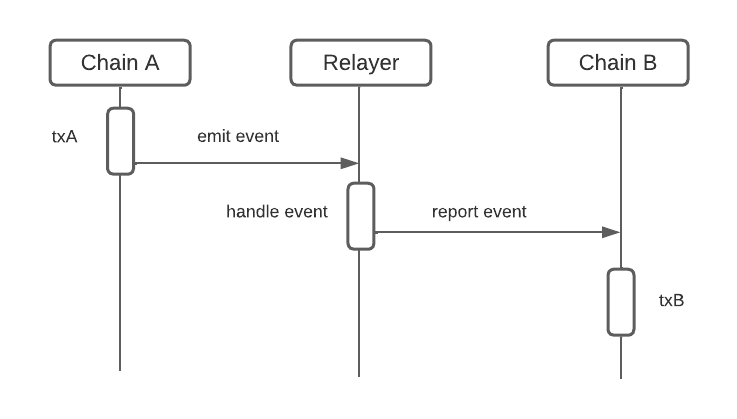
\includegraphics[scale=0.6]{relayer}
\caption{Forwarding message using a relayer}
\label{relayer-connection}
\end{figure}

\subsection{Technical Challenges}
The major security challenge regarding the above model is that we require the relayer to be honest and authorized. A centralized relayer can be built such that chain B only accepts information reported from a trusted relayer. In such a solution, safety is enforced since the trusted relayer signs all their messages with their private key and $tx_B$ in chain B checks the signature accordingly. However with such a centralized setup, the relayer becomes one of the most important trust bases for the protocol to work which may lead to SIOF (single point of failure) if the relayer is hacked or misbehaved.

%This built-in drawback of blockchains makes it hard to execute a group of transactions involving different chains so that either all of them or none of them succeed on different chains. 

To take a step further, we consider two bundled transactions $T_1$ and $T_2$. $T_1$ contains $tx_A^1$ on blockchain $C_A$ and $tx_B^1$ on blockchain $C_B$. $T_2$ contains $tx^2_C$ on blockchain $C_C$ and $tx_B^1$ on blockchain $C_B$. Then it follows that the safety property requires transactions in $T_1$ and $T_2$ both succeed or none of them succeed. In such senario, the safety of relayer does not enforce the safety of the bundled transactions as there might be interference between the execution of $T_1$ and $T_2$ (e.g. the execution sequence is $tx_A^1$, $tx_C^2$, $tx_B^1$, $tx_B^2$). 

Suppose that a protocol is designed to help carry out such bundled transactions between blockchains, then we can define the safety, permissionless, liveness, and linearizability properties of the protocol as follows:

\smallskip\noindent\emph{Permissionless.} Any nodes of a certain blockchain are allowed to join the communication network.

\smallskip\noindent\emph{Safety.} All state updates for a single transaction are either successful or fail on all involved blockchains.

\smallskip\noindent\emph{Liveness.} All valid transactions will eventually succeed on all blockchains.

\smallskip\noindent\emph{Linearizability.} All concurrent successful transactions are always linearizable so that the consequent state of a group of concurrent transactions $tx_i$ is equivalent to performing the transactions sequentially in a special order that respects the happen-before relation of the original order.

Although various solutions tried to tackle the above problems, they usually restricted the scope of use-cases to be transactions within two blockchains where the atomicity and liveness properties is simpler comparing to multi-chain scenarios.

Recently the development of PCS (Polynomial Commitment schemes) provides a new way to convince others that the polynomial has certain evaluation at certain point without redo the calculation. Based on this technique, ZKSNARK (Zero-Knowledge Succinct Non-Interactive Argument of Knowledge) become technically mature which is often used to prove that a statement is true, without revealing any information beyond the validity of the statement itself. Some usage of ZKSNARK in cross-chain communication can be found in \cite{sidechainzkp, cao2020-zk-atomic, garoffolo2020zendoo} which still mainly focus on communications between two blockchains by providing a secure (ZKP backed) relayer.

\subsection{Our Contribution}

In this paper, we make the following contributions:
\begin{itemize}
\item We consider the general case of multi-chain bundled transactions and provide a novel way to preserve the linearizability of transactions cross multiple blockchains. In particular, instead of executing multiple transactions on different blockchains and using relayers to synchronize them, we simulate the transactions on our aggregation layer and generate ZKP (zero-knowledge-proofs) to convince involved blockchains to update their state accordingly afterwards. \\

\item Our approach not only enforces linearizability natually, but also allows transaction be designed to have a view of multichain states. For example, if a traditional two-chain transaction contains $t_1$ and $t_2$ then $t_1$ can only see the state on blockchain $C_1$ and $t_2$ can only see the state of blockchain $C_2$. By using our approach, $t_1$ and $t_2$ can both see the global state of $C_1 \times C_2$.\\

\item We provide a permissionless solution by encoding the consensus algorithm into ZKP. By doing so we get the following benefits.
\begin{itemize}
    \item Compares to other solutions which requires the up bound number of monitors are fixed, our solution allows new anonymous nodes to register them-self into the system. We believe that only by providing a dynamic relayer system, the liveness property is enforced.
    \item We allow user to trigger bundled transactions not only on native blockchain but also on our aggregator chain which was technically hard as we need to prevent dishonest nodes that systemically ignore transactions triggered on aggregator chain.
    \end{itemize}
\end{itemize}